\chapter{Results} 
\label{Chapter5}

This chapter details the results and findings attained throughout this project. First, The feature selection results for each of the datasets used to train the 28 models are displayed. Second, the performance of each of the models are displayed are discussed. Finally, this chapter discusses if the alternative data features used throughout this project improved model performance.  

%%%%%%%%%%%%%%%%%%%%%%%%%%%%%%%%%%%%%%%

\section{Features Selected for Each Dataset}

For each of the data category combinations shown in Section 4.1, RFE is used to identify the most relevant features, while cross validation is used to validate the optimal number of features used. Figures \ref{fig:sd}, \ref{fig:cb}, and \ref{fig:alt} display the number of features against model accuracy for datasets containing only sociodemographic, credit bureau, and alternative features respectively. Figure \ref{fig:all} displays the number of features against model accuracy for the dataset containing all 3 category combinations. \\


The figures highlight the variation in model accuracy and the importance of feature selection. Figure \ref{fig:sd} displays a spike in accuracy when only 2 SD features are used, but then a gradual increase in accuracy as more SD features are added to the feature space. Figure \ref{fig:cb} displays that there is a decrease in accuracy when more CB features are added to the features space, until the number of features moves beyond 5. Figure \ref{fig:alt} displays that once the number of alternative data features moves beyond 8, there is either very little increase in accuracy or the accuracy decreases. While, Figure \ref{fig:all} displays that model accuracy improves rapidly when features are first added to the feature space, then after 10 feautes accruacy gradually increases until 43 features are in the feature space. 


\vspace{10 pt}

\begin{figure}[!htb]
\centering
  \begin{minipage}{0.5\textwidth}
    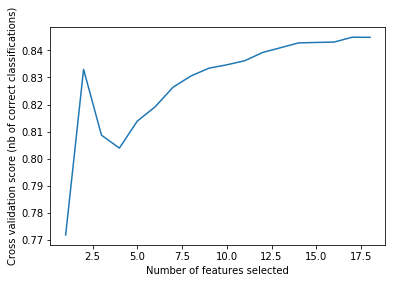
\includegraphics[width=\textwidth]{images/sd_only.png}
    \caption{Sociodemographic Variable Selection}
    \label{fig:sd}
  \end{minipage}%
  \begin{minipage}{0.5\textwidth}
    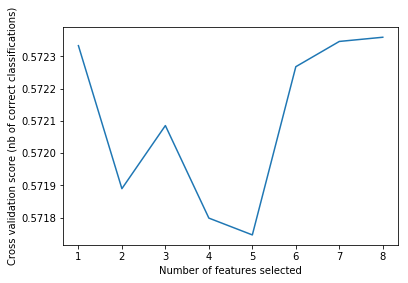
\includegraphics[width=\textwidth]{images/cb_only.png}
    \caption{Credit Bureau Variable Selection}
    \label{fig:cb}
  \end{minipage}
\end{figure}

\newpage

\vspace{10 pt}

\begin{figure}[!htb]
\centering
  \begin{minipage}{0.5\textwidth}
    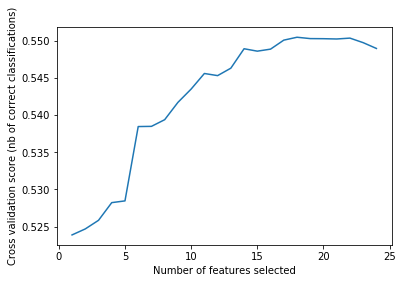
\includegraphics[width=\textwidth]{images/alt_only.png}
    \caption{Alternative Data Variable Selection}
    \label{fig:alt}
  \end{minipage}%
  \begin{minipage}{0.5\textwidth}
    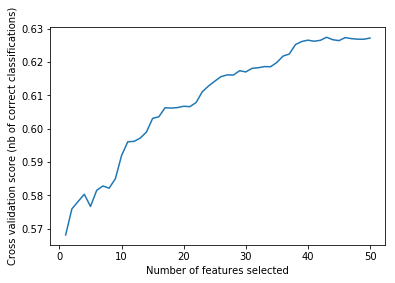
\includegraphics[width=\textwidth]{images/sd_cb_alt.png}
    \caption{Variable Selection for the All Datasets}
    \label{fig:all}
  \end{minipage}
\end{figure}

\vspace{10 pt}


Table \ref{table:features retained} displays the feature selection results for all 7 category combinations. The table provides the number of features each dataset, the number of features selected from each dataset, and the names of the features that were deemed irrelevant. \\

The table highlights a mass drop of features when only CB and ALD features are used. This could indicate dependencies and collinearity between variables in that dataset, however the difference between the lowest and highest validation accuracies is was last than 1\%.  \\

Furthermore, the Table validates the trends displayed in Figures \ref{fig:sd}, \ref{fig:cb}, \ref{fig:alt}, and \ref{fig:all}. This is particular evident in the ALD row. \\

It can be noted that the variables appear to be consistently removed by the RFE process. For example income is removed in the SD; SD and CB; SD and ALD; and SD, CB, and ALD datasets. The same pattern can be extended for many of the ALD and CB variables.  

\vspace{10pt}

\begin{longtable}{|p{3cm}|p{2cm}|p{2cm}|p{6cm}|} 
\hline
\multicolumn{1}{|p{3cm}|}{Dataset}
&\multicolumn{1}{|p{2cm}|}{Features}
&\multicolumn{1}{|p{2cm}|}{Selected Features}
&\multicolumn{1}{|p{6cm}|}{Features Not Selected}\\
\hline
SD & 18 & 16 & income   \\
\hline
CB & 8 & 8 &   \\
\hline
ALD & 24 & 8  & competitor count, gambling count, app count, max balance, max credit, max debit, min debit, insufficient funds,  successful payments, max successful loan payment, min  successful loan payment, unsuccessful payments, max unsuccessful loan payment, min unsuccessful loan payment, rejected loans, max loan amount \\
\hline
SD and CB & 26 & 21 & property status, time at employer , application time , application week , income \\
\hline
SD and ALD & 42 & 39 & income, competitor count, gambling count \\
\hline
CB and ALD & 32 & 3 &  open accounts by date, performing loans, paid loans, nonperforming loans, lost loans, missed payments, competitor count, banking count, news count, gambling count, VPN count, app count, device price, max balance, min balance, credit transactions, max credit, min credit, max debit, min debit, insufficient funds, successful payments, max successful loan payment, min successful loan payment, unsuccessful payments, max unsuccessful loan payment, min unsuccessful loan payment, rejected loans, max loan amount \\
\hline
SD, CB and ALD & 50 & 43 & application week, income, lost loans, competitor count, gambling count, insufficient funds, min unsuccessful loan payment\\
\hline
\caption{Feature Selection Results}
\label{table:features retained}
\end{longtable}

%%%%%%%%%%%%%%%%%%%%%%%%%%%%%%%%%%%%%%%

\section{Logistic Regression}

\vspace{10pt}

\begin{table}[H]
\begin{center}
\begin{tabular}{|c|c|c|c|c|c|} 
\hline
\multicolumn{1}{|c|}{Dataset}
&\multicolumn{1}{|c|}{Accuracy}
&\multicolumn{1}{|c|}{Repaid Accuracy}
&\multicolumn{1}{|c|}{Default Accuracy}
&\multicolumn{1}{|c|}{F1 Score}
&\multicolumn{1}{|c|}{AUC}\\
\hline
SD & 0.58 & 0.55 & 0.58 & 0.58 & 0.61    \\
\hline
CB & 0.57 & 0.39 & 0.76 & 0.57 & 0.60    \\
\hline
ALD & 0.54 & 0.46 & 0.62 & 0.54 & 0.56    \\
\hline
SD and CB & 0.60 & 0.60 & 0.61 & 0.60 & 0.65    \\
\hline
SD and ALD & 0.61 & 0.64 & 0.59 & 0.61 & 0.66    \\
\hline
CB and ALD & 0.58 & 0.44 & 0.75 & 0.59 & 0.61    \\
\hline
SD, CB and ALD & 0.63 & 0.62 & 0.64 & 0.63 & 0.68    \\
\hline
\end{tabular}
\end{center}
\caption{Logistic Regression Training Performance}
\label{table:lr training}
\end{table}

\vspace{10pt}

\begin{table}[H]
\begin{center}
\begin{tabular}{|c|c|c|c|c|c|} 
\hline
\multicolumn{1}{|c|}{Dataset}
&\multicolumn{1}{|c|}{Accuracy}
&\multicolumn{1}{|c|}{Precision}
&\multicolumn{1}{|c|}{Recall}
&\multicolumn{1}{|c|}{F1 Score}
&\multicolumn{1}{|c|}{AUC}\\
\hline
SD & 0.61 & 0.62 & 0.55 & 0.61 & 0.63    \\
\hline
CB & 0.48 & 0.40 & 0.75 & 0.48 & 0.62    \\
\hline
ALD & 0.50 & 0.47 & 0.64 & 0.51 & 0.57    \\
\hline
SD and CB & 0.61 & 0.61 & 0.62 & 0.61 & 0.65    \\
\hline
SD and ALD & 0.63 & 0.64 & 0.59 & 0.63 & 0.66    \\
\hline
CB and ALD & 0.51 & 0.43 & 0.73 & 0.53 & 0.62    \\
\hline
SD, CB and ALD & 0.64 & 0.64 & 0.63 & 0.63 & 0.68    \\
\hline
\end{tabular}
\end{center}
\caption{Logistic Regression Validation Performance}
\label{table:lr test}
\end{table}

\vspace{10pt}

%%%%%%%%%%%%%%%%%%%%%%%%%%%%%%%%%%%%%%%


\section{Random Forest}

\vspace{10pt}

\begin{table}[H]
\begin{center}
\begin{tabular}{|c|c|c|c|c|c|} 
\hline
\multicolumn{1}{|c|}{Dataset}
&\multicolumn{1}{|c|}{Accuracy}
&\multicolumn{1}{|c|}{Precision}
&\multicolumn{1}{|c|}{Recall}
&\multicolumn{1}{|c|}{F1 Score}
&\multicolumn{1}{|c|}{AUC}\\
\hline
SD & 0.81 & 0.82 & 0.81 & 0.82 & 0.83    \\
\hline
CB & 0.63 & 0.53 & 0.74 & 0.63 & 0.68    \\
\hline
ALD & 0.71 & 0.74 & 0.69 & 0.71 & 0.80    \\
\hline
SD and CB & 0.83 & 0.83 & 0.83 & 0.83 & 0.88    \\
\hline
SD and ALD & 0.85 & 0.86 & 0.85 & 0.85 & 0.92    \\
\hline
CB and ALD & 0.69 & 0.68 & 0.71 & 0.70 & 0.78    \\
\hline
SD, CB and ALD & 0.87 & 0.87 & 0.87 & 0.87 & 0.93    \\
\hline
\end{tabular}
\end{center}
\caption{Random Forest Training Performance}
\label{table:rf training}
\end{table}

\vspace{10pt}

\begin{table}[H]
\begin{center}
\begin{tabular}{|c|c|c|c|c|c|} 
\hline
\multicolumn{1}{|c|}{Dataset}
&\multicolumn{1}{|c|}{Accuracy}
&\multicolumn{1}{|c|}{Precision}
&\multicolumn{1}{|c|}{Recall}
&\multicolumn{1}{|c|}{F1 Score}
&\multicolumn{1}{|c|}{AUC}\\
\hline
SD & 0.71 & 0.81 & 0.37 & 0.70 & 0.60    \\
\hline
CB & 0.56 & 0.52 & 0.68 & 0.56 & 0.63    \\
\hline
ALD & 0.66 & 0.72 & 0.44 & 0.66 & 0.62    \\
\hline
SD and CB & 0.73 & 0.83 & 0.39 & 0.73 & 0.66    \\
\hline
SD and ALD & 0.79 & 0.86 & 0.53 & 0.78 & 0.80    \\
\hline
CB and ALD & 0.64 & 0.68 & 0.47 & 0.64 & 0.60    \\
\hline
SD, CB and ALD & 0.80 & 0.87 & 0.54 & 0.79 & 0.81    \\
\hline
\end{tabular}
\end{center}
\caption{Random Forest Validation Performance}
\label{table:rf test}
\end{table}

\vspace{10pt}


%%%%%%%%%%%%%%%%%%%%%%%%%%%%%%%%%%%%%%%


\section{Extreme Gradient Boosting}

\vspace{10pt}

\begin{table}[H]
\begin{center}
\begin{tabular}{|c|c|c|c|c|c|} 
\hline
\multicolumn{1}{|c|}{Dataset}
&\multicolumn{1}{|c|}{Accuracy}
&\multicolumn{1}{|c|}{Precision}
&\multicolumn{1}{|c|}{Recall}
&\multicolumn{1}{|c|}{F1 Score}
&\multicolumn{1}{|c|}{AUC}\\
\hline
SD & 0.81 & 0.82 & 0.81 & 0.82 & 0.83    \\
\hline
CB & 0.63 & 0.53 & 0.74 & 0.63 & 0.68    \\
\hline
ALD & 0.71 & 0.74 & 0.69 & 0.71 & 0.80    \\
\hline
SD and CB & 0.83 & 0.83 & 0.83 & 0.83 & 0.88    \\
\hline
SD and ALD & 0.85 & 0.86 & 0.85 & 0.85 & 0.92    \\
\hline
CB and ALD & 0.69 & 0.68 & 0.71 & 0.70 & 0.78    \\
\hline
SD, CB and ALD & 0.87 & 0.87 & 0.87 & 0.87 & 0.93    \\
\hline
\end{tabular}
\end{center}
\caption{XGBoost Training Performance}
\label{table:xgb training}
\end{table}

\vspace{10pt}

\begin{table}[H]
\begin{center}
\begin{tabular}{|c|c|c|c|c|c|} 
\hline
\multicolumn{1}{|c|}{Dataset}
&\multicolumn{1}{|c|}{Accuracy}
&\multicolumn{1}{|c|}{Precision}
&\multicolumn{1}{|c|}{Recall}
&\multicolumn{1}{|c|}{F1 Score}
&\multicolumn{1}{|c|}{AUC}\\
\hline
SD & 0.71 & 0.81 & 0.37 & 0.70 & 0.60    \\
\hline
CB & 0.56 & 0.52 & 0.68 & 0.56 & 0.63    \\
\hline
ALD & 0.66 & 0.72 & 0.44 & 0.66 & 0.62    \\
\hline
SD and CB & 0.73 & 0.83 & 0.39 & 0.73 & 0.66    \\
\hline
SD and ALD & 0.79 & 0.86 & 0.53 & 0.78 & 0.80    \\
\hline
CB and ALD & 0.64 & 0.68 & 0.47 & 0.64 & 0.60    \\
\hline
SD, CB and ALD & 0.80 & 0.87 & 0.54 & 0.79 & 0.81    \\
\hline
\end{tabular}
\end{center}
\caption{XGBoost Validation Performance}
\label{table:xgb test}
\end{table}

\vspace{10pt}